\section{未命名节}

\subsection{统计工具}

\section{ 统计工具}

\subsection{8.1.1 统计工具}
\begin{center}
\Large \textcolor{blue}{如何用数学语言描述"用历史预测未来"?}
\end{center}


\paragraph{自回归模型(Autoregressive Model)}
\textbf{核心思想:}当前时刻的值依赖于过去的值

\begin{definition}[数学定义]
$$x_t = f(x_{t-1}, x_{t-2}, \ldots, x_{t-\tau}) + \epsilon_t$$
\end{definition}

\textbf{符号说明:}
\begin{itemize}
    \item $x_t$:时间步 $t$ 的观测值(我们要预测的)
    \item $x_{t-1}, x_{t-2}, \ldots, x_{t-\tau}$:过去 $\tau$ 个时间步的值
    \item $f(\cdot)$:某个函数(可以是线性、非线性、神经网络...)
    \item $\epsilon_t$:随机噪声项
    \item $\tau$:\textbf{回顾窗口}(look-back window)的大小
\end{itemize}

\begin{theorem}[名字的由来]
\textbf{Auto}(自己)+ \textbf{Regressive}(回归)= 用自己的历史值来回归
\end{theorem}


\paragraph{简单例子:线性自回归(AR模型)}
\textbf{假设:}未来是过去的加权平均

$$x_t = w_1 x_{t-1} + w_2 x_{t-2} + w_3 x_{t-3} + b + \epsilon_t$$

\begin{example}[具体数值例子]
假设我们预测股价,学到的参数是:
$$x_t = 0.5 x_{t-1} + 0.3 x_{t-2} + 0.2 x_{t-3} + 1.0$$

如果 $x_{t-1}=100$, $x_{t-2}=98$, $x_{t-3}=95$,则:
$$x_t = 0.5 \times 100 + 0.3 \times 98 + 0.2 \times 95 + 1.0 = 99.4$$
\end{example}

\begin{center}
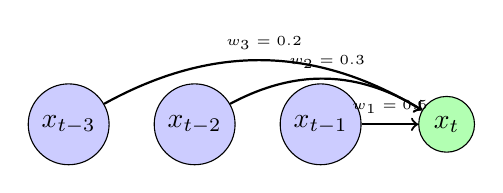
\begin{tikzpicture}[scale=0.8]
\node[circle,draw,fill=blue!20] (x1) at (0,0) {$x_{t-3}$};
\node[circle,draw,fill=blue!20] (x2) at (2,0) {$x_{t-2}$};
\node[circle,draw,fill=blue!20] (x3) at (4,0) {$x_{t-1}$};
\node[circle,draw,fill=green!30] (xt) at (6,0) {$x_t$};

\draw[->,thick] (x1) to[bend left] node[above,font=\tiny] {$w_3=0.2$} (xt);
\draw[->,thick] (x2) to[bend left] node[above,font=\tiny] {$w_2=0.3$} (xt);
\draw[->,thick] (x3) -- node[above,font=\tiny] {$w_1=0.5$} (xt);
\end{tikzpicture}
\end{center}


\paragraph{自回归模型的问题}
\begin{theorem}[问题1:窗口大小 $\tau$ 如何选择?]
\begin{itemize}
    \item $\tau$ 太小:丢失长期信息,如季节性规律
    \item $\tau$ 太大:参数太多,计算复杂,过拟合
\end{itemize}
\end{theorem}




\begin{definition}[理想情况]
我们希望:\textbf{参数数量固定},但能\textbf{记住所有历史}!
\end{definition}


\paragraph{隐变量自回归模型}
\textbf{关键思想:}引入一个\textbf{隐变量}(hidden state)$h_t$ 来总结历史

\begin{definition}[数学形式]
\begin{align*}
h_t &= g(h_{t-1}, x_{t-1}) \quad \text{\textcolor{blue}{(更新记忆)}}\\
x_t &= f(h_t) + \epsilon_t \quad \text{\textcolor{red}{(生成预测)}}
\end{align*}
\end{definition}

\textbf{直观理解:}
\begin{itemize}
    \item $h_t$:像大脑的\textbf{记忆},存储到时刻 $t$ 的所有重要信息
    \item $g$:\textbf{更新函数},根据新观测 $x_{t-1}$ 更新记忆
    \item $f$:\textbf{输出函数},根据当前记忆预测未来
\end{itemize}

\begin{center}
\begin{tikzpicture}[scale=1.1]
\node[circle,draw,fill=red!20,minimum size=1cm] (h1) at (0,1.5) {$h_1$};
\node[circle,draw,fill=red!20,minimum size=1cm] (h2) at (2,1.5) {$h_2$};
\node[circle,draw,fill=red!20,minimum size=1cm] (h3) at (4,1.5) {$h_3$};
\node[circle,draw,fill=red!20,minimum size=1cm] (h4) at (6,1.5) {$h_4$};

\node[circle,draw,fill=blue!20] (x1) at (0,0) {$x_1$};
\node[circle,draw,fill=blue!20] (x2) at (2,0) {$x_2$};
\node[circle,draw,fill=blue!20] (x3) at (4,0) {$x_3$};
\node[circle,draw,fill=green!30] (x4) at (6,0) {$x_4$};

\draw[->,thick] (x1) -- (h1);
\draw[->,thick] (x2) -- (h2);
\draw[->,thick] (x3) -- (h3);
\draw[->,thick] (h1) -- (h2) node[midway,above,font=\tiny] {$g$};
\draw[->,thick] (h2) -- (h3) node[midway,above,font=\tiny] {$g$};
\draw[->,thick] (h3) -- (h4) node[midway,above,font=\tiny] {$g$};
\draw[->,thick] (h4) -- (x4) node[midway,right,font=\tiny] {$f$};

\node[below,font=\small] at (3,-0.7) {隐状态像"记忆",不断更新};
\end{tikzpicture}
\end{center}


\paragraph{隐变量模型的优势}


\textbf{标准自回归:}
\begin{center}
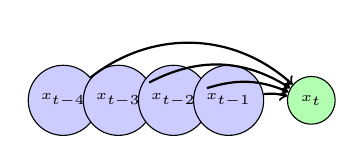
\begin{tikzpicture}[scale=0.7]
\node[circle,draw,fill=blue!20,font=\tiny] (x1) at (0,0) {$x_{t-4}$};
\node[circle,draw,fill=blue!20,font=\tiny] (x2) at (1,0) {$x_{t-3}$};
\node[circle,draw,fill=blue!20,font=\tiny] (x3) at (2,0) {$x_{t-2}$};
\node[circle,draw,fill=blue!20,font=\tiny] (x4) at (3,0) {$x_{t-1}$};
\node[circle,draw,fill=green!30,font=\tiny] (xt) at (4.5,0) {$x_t$};

\draw[->,thick] (x1) to[bend left=40] (xt);
\draw[->,thick] (x2) to[bend left=30] (xt);
\draw[->,thick] (x3) to[bend left=20] (xt);
\draw[->,thick] (x4) to[bend left=10] (xt);
\end{tikzpicture}
\end{center}

\textcolor{red}{\textbf{问题:}}
\begin{itemize}
    \item 输入维度 = $\tau$
    \item 历史越长,输入越大
    \item 参数数量:$\tau \times d$
\end{itemize}


\textbf{隐变量模型:}
\begin{center}
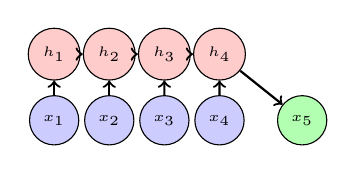
\begin{tikzpicture}[scale=0.7]
\node[circle,draw,fill=red!20,font=\tiny] (h1) at (0,1.2) {$h_1$};
\node[circle,draw,fill=red!20,font=\tiny] (h2) at (1,1.2) {$h_2$};
\node[circle,draw,fill=red!20,font=\tiny] (h3) at (2,1.2) {$h_3$};
\node[circle,draw,fill=red!20,font=\tiny] (h4) at (3,1.2) {$h_4$};

\node[circle,draw,fill=blue!20,font=\tiny] (x1) at (0,0) {$x_1$};
\node[circle,draw,fill=blue!20,font=\tiny] (x2) at (1,0) {$x_2$};
\node[circle,draw,fill=blue!20,font=\tiny] (x3) at (2,0) {$x_3$};
\node[circle,draw,fill=blue!20,font=\tiny] (x4) at (3,0) {$x_4$};
\node[circle,draw,fill=green!30,font=\tiny] (x5) at (4.5,0) {$x_5$};

\foreach \i in {1,2,3,4} {
    \draw[->,thick] (x\i) -- (h\i);
}
\draw[->,thick] (h1) -- (h2);
\draw[->,thick] (h2) -- (h3);
\draw[->,thick] (h3) -- (h4);
\draw[->,thick] (h4) -- (x5);
\end{tikzpicture}
\end{center}

\textcolor{blue}{\textbf{优势:}}
\begin{itemize}
    \item 输入维度固定
    \item 无论历史多长
    \item 参数数量不变
\end{itemize}


\vspace{0.5cm}
\begin{theorem}[关键创新]
$h_t$ 就像一个\textbf{压缩包},把所有历史信息压缩存储!\\
这就是\textbf{循环神经网络(RNN)}的核心思想!
\end{theorem}


\paragraph{隐状态的直观类比}
\begin{center}
\begin{tikzpicture}[scale=1.1]
% 人脑
%\node[inner sep=0] at (0,2) {\includegraphics[width=1.5cm]{brain.png}};
\node[below,text width=3cm,align=center] at (0,0.8) {
\textbf{人类记忆}\\
看到新信息\\
$\downarrow$\\
更新记忆\\
$\downarrow$\\
基于记忆决策
};

% 箭头
\draw[->,ultra thick] (1.5,2) -- (3.5,2);

% 隐状态
\node[circle,draw,fill=red!30,minimum size=1.5cm] at (5,2) {$h_t$};
\node[below,text width=3cm,align=center] at (5,0.8) {
\textbf{隐状态}\\
观测到 $x_{t-1}$\\
$\downarrow$\\
更新 $h_t = g(h_{t-1}, x_{t-1})$\\
$\downarrow$\\
预测 $x_t = f(h_t)$
};

% 箭头
\draw[->,ultra thick] (6.5,2) -- (8.5,2);

% RNN
%\node[inner sep=0] at (10,2) {\includegraphics[width=1.5cm]{rnn.png}};
\node[below,text width=3cm,align=center] at (10,0.8) {
\textbf{循环神经网络}\\
实现隐状态\\
的具体架构
};

\end{tikzpicture}
\end{center}

\begin{definition}[类比]
隐状态 $h_t$ = 你看完前面所有剧集后的记忆\\
你不记得每一个细节,但记得关键信息!
\end{definition}



\subsection{训练}

\section{8.1.2 训练}

\paragraph{ 训练序列模型}
\begin{center}
\Large \textcolor{blue}{有了模型,如何从数据中学习参数?}
\end{center}


\paragraph{训练的基本思路}
\textbf{给定:}训练序列 $x_1, x_2, x_3, \ldots, x_T$

\textbf{目标:}找到最优参数,使模型预测尽可能准确

\begin{definition}[训练三步骤]
\begin{enumerate}
    \item \textbf{定义模型}:选择 $f$ 和 $g$ 的具体形式
    \item \textbf{定义损失函数}:衡量预测与真实值的差距
    \item \textbf{优化参数}:用梯度下降最小化损失
\end{enumerate}
\end{definition}

\begin{center}
\begin{tikzpicture}[scale=1.0]
\node[draw,fill=yellow!20,rounded corners,text width=2.5cm,align=center] at (0,0) {
训练数据\\
$\{x_1, \ldots, x_T\}$
};

\draw[->,thick] (1.5,0) -- (2.5,0);

\node[draw,fill=blue!20,rounded corners,text width=2cm,align=center] at (4,0) {
模型\\
$x_t = f_\theta(x_{<t})$
};

\draw[->,thick] (5.5,0) -- (6.5,0);

\node[draw,fill=red!20,rounded corners,text width=2cm,align=center] at (8,0) {
损失函数\\
$L(\theta)$
};

\draw[->,thick] (8,-0.8) -- (4,-0.8);
\node[below,font=\small] at (6,-1) {梯度下降优化};
\end{tikzpicture}
\end{center}


\paragraph{例子:训练线性自回归模型}
\textbf{模型:}$x_t = w_1 x_{t-1} + w_2 x_{t-2} + b$

\textbf{损失:}均方误差 $L = \frac{1}{T}\sum_{t=1}^{T}(x_t - \hat{x}_t)^2$

% \begin{lstlisting}
% import torch
% import torch.nn as nn
% 
% # Generate simulated data( + )
% T = 1000
% time = torch.arange(1, T + 1, dtype=torch.float32)
% x = torch.sin(0.01 * time) + torch.randn(T) * 0.2
% 
% # Prepare training datausing2time steppredictionnext step
% tau = 2
% features = torch.zeros((T - tau, tau))
% for i in range(tau):
%     features[:, i] = x[i: T - tau + i]
% labels = x[tau:].reshape((-1, 1))
% 
% # Define linear model
% model = nn.Linear(tau, 1)
% loss_fn = nn.MSELoss()
% optimizer = torch.optim.SGD(model.parameters(), lr=0.01)
% \end{lstlisting}


\paragraph{训练循环}
\begin{lstlisting}
# training
num_epochs = 10
for epoch in range(num_epochs):
    predictions = model(features)
    loss = loss_fn(predictions, labels)
    
    optimizer.zero_grad()
    loss.backward()
    optimizer.step()
    
    if (epoch + 1) % 2 == 0:
        print(f'Epoch {epoch+1}, Loss: {loss.item():.4f}')

# Output
# Epoch 2, Loss: 0.0523
# Epoch 4, Loss: 0.0418
# Epoch 6, Loss: 0.0387
# Epoch 8, Loss: 0.0372
# Epoch 10, Loss: 0.0365
\end{lstlisting}

\begin{definition}[训练过程]
损失逐渐下降 $\to$ 模型学到了数据的规律
\end{definition}


\section{8.1.3 预测}

\subsection{8.1.3 预测}
\begin{center}
\Large \textcolor{blue}{训练完模型后,如何用它来预测?}
\end{center}


\paragraph{单步预测 vs 多步预测}


\textbf{单步预测(One-step Ahead):}
\begin{center}
\begin{tikzpicture}[scale=0.8]
\foreach \i in {1,...,5} {
    \node[circle,draw,fill=blue!20,font=\tiny] (x\i) at (\i*0.8,0) {$x_{\i}$};
}
\node[circle,draw,fill=green!30,font=\tiny] (x6) at (5.6,0) {$\hat{x}_6$};

\draw[->,thick,red] (x5) -- (x6);
\draw[decorate,decoration={brace,amplitude=5pt},thick] (0.4,-0.5) -- (4.4,-0.5);
\node[below] at (2.4,-0.7) {\tiny 已知};
\node[below,green!60!black] at (5.6,-0.5) {\tiny 预测};
\end{tikzpicture}
\end{center}

\textbf{特点:}
\begin{itemize}
    \item 只预测\textbf{下一步}
    \item 使用\textbf{真实}历史数据
    \item 准确度高
\end{itemize}


\textbf{多步预测(Multi-step Ahead):}
\begin{center}
\begin{tikzpicture}[scale=0.8]
\foreach \i in {1,2,3} {
    \node[circle,draw,fill=blue!20,font=\tiny] (x\i) at (\i*0.8,0) {$x_{\i}$};
}
\foreach \i in {4,5,6} {
    \node[circle,draw,fill=green!30,font=\tiny] (x\i) at (\i*0.8,0) {$\hat{x}_{\i}$};
}

\draw[->,thick,red] (x3) -- (x4);
\draw[->,thick,red] (x4) -- (x5);
\draw[->,thick,red] (x5) -- (x6);
\draw[decorate,decoration={brace,amplitude=5pt},thick] (0.4,-0.5) -- (2.6,-0.5);
\node[below] at (1.5,-0.7) {\tiny 已知};
\node[below,green!60!black] at (4.4,-0.5) {\tiny 多步预测};
\end{tikzpicture}
\end{center}

\textbf{特点:}
\begin{itemize}
    \item 预测\textbf{未来多步}
    \item 使用\textbf{预测值}作输入
    \item 误差会累积
\end{itemize}


\vspace{0.5cm}
\begin{theorem}[核心区别]
单步预测:$\hat{x}_{t+1} = f(x_t, x_{t-1}, \ldots)$ $\leftarrow$ 用真实值\\
多步预测:$\hat{x}_{t+k} = f(\hat{x}_{t+k-1}, \hat{x}_{t+k-2}, \ldots)$ $\leftarrow$ 用预测值
\end{theorem}


\paragraph{多步预测的误差累积}
\begin{center}
\begin{tikzpicture}[scale=1.1]
% 时间轴
\draw[->,thick] (0,0) -- (9,0) node[right] {时间步};
\draw[->,thick] (0,0) -- (0,3.5) node[above] {值};

% 真实值(蓝色实线)
\draw[blue,thick] (1,1.5) -- (2,1.8) -- (3,2.0) -- (4,1.9) -- (5,2.1) -- (6,2.3) -- (7,2.2) -- (8,2.4);
\foreach \x/\y in {1/1.5, 2/1.8, 3/2.0, 4/1.9, 5/2.1, 6/2.3, 7/2.2, 8/2.4} {
    \fill[blue] (\x,\y) circle (2pt);
}

% 预测值(红色虚线,误差越来越大)
\draw[red,thick,dashed] (3,2.0) -- (4,1.85) -- (5,1.95) -- (6,1.9) -- (7,1.7) -- (8,1.5);
\foreach \x/\y in {4/1.85, 5/1.95, 6/1.9, 7/1.7, 8/1.5} {
    \fill[red] (\x,\y) circle (2pt);
}

% 标注
\draw[blue,thick] (0.5,3.2) -- (1.5,3.2) node[right,black] {真实值};
\draw[red,thick,dashed] (0.5,2.8) -- (1.5,2.8) node[right,black] {预测值};

% 误差标注
\draw[<->,thick,purple] (6,2.3) -- (6,1.9) node[midway,right] {\tiny 误差};
\draw[<->,thick,purple] (8,2.4) -- (8,1.5) node[midway,right] {\tiny 累积误差};

% 分界线
\draw[thick,green!60!black,dashed] (3,-0.3) -- (3,3);
\node[below,green!60!black] at (3,-0.3) {预测起点};
\end{tikzpicture}
\end{center}

\begin{theorem}[误差累积现象]
\begin{itemize}
    \item 第1步预测有小误差 $\epsilon_1$
    \item 第2步基于有误差的预测,误差变大 $\epsilon_1 + \epsilon_2$
    \item 第3步误差继续累积...
    \item 预测越远,误差越大!
\end{itemize}
\end{theorem}


\paragraph{单步预测代码示例}
\begin{lstlisting}
# Single-step prediction using real historical data
def predict_one_step(model, x_history, tau):
    """ x_history: shape (tau,) Return: next step prediction """
    with torch.no_grad():
        x_input = x_history[-tau:].reshape(1, -1)
        prediction = model(x_input)
    return prediction.item()

x_true = torch.tensor([1.0, 1.2, 1.1, 1.3, 1.2])
next_value = predict_one_step(model, x_true, tau=2)
print(f"Based on {x_true[-2:].tolist()} predict: {next_value:.3f}")

# Output
# Based on [1.3, 1.2] predict: 1.245
\end{lstlisting}

\begin{definition}[关键]
使用\textbf{真实的}历史数据 $x_{t-1}, x_{t-2}, \ldots$ 作为输入
\end{definition}


\paragraph{多步预测:递归策略}
\begin{lstlisting}
# Multi-step prediction using recursive strategy
def predict_multi_step(model, x_history, tau, k_steps):
    """ x_history: initial history data, shape (tau,) k_steps: number of steps to predict Return: k prediction values """
    predictions = []
    current_input = x_history[-tau:].clone()
    
    for _ in range(k_steps):
        # Predict next step
        with torch.no_grad():
            next_pred = model(current_input.reshape(1, -1))
        predictions.append(next_pred.item())
        
        # Update input with prediction
        current_input = torch.cat([current_input[1:], 
                                   next_pred.reshape(1)])
    
    return predictions

predictions = predict_multi_step(model, x_true, tau=2, k_steps=5)
print(f"Future 5-step predictions: {predictions}")
# Output: Future 5-step predictions: [1.245, 1.233, 1.239, 1.236, 1.237]
\end{lstlisting}


\paragraph{多步预测的可视化}
\begin{center}
\begin{tikzpicture}[scale=1.0]
% 标题
\node[font=\large\bfseries] at (5,4) {递归多步预测过程};

% 步骤1
\node[draw,fill=blue!20,text width=8cm] at (5,3) {
\textbf{步骤1:} 用真实历史 $[x_3, x_4]$ $\to$ 预测 $\hat{x}_5$
};

% 步骤2
\node[draw,fill=yellow!20,text width=8cm] at (5,2) {
\textbf{步骤2:} 用 $[x_4, \hat{x}_5]$ $\to$ 预测 $\hat{x}_6$
};

% 步骤3
\node[draw,fill=orange!20,text width=8cm] at (5,1) {
\textbf{步骤3:} 用 $[\hat{x}_5, \hat{x}_6]$ $\to$ 预测 $\hat{x}_7$
};

% 步骤4
\node[draw,fill=red!20,text width=8cm] at (5,0) {
\textbf{步骤4:} 用 $[\hat{x}_6, \hat{x}_7]$ $\to$ 预测 $\hat{x}_8$
};

% 箭头
\foreach \y in {2.5,1.5,0.5} {
    \draw[->,ultra thick] (5,\y+0.3) -- (5,\y-0.3);
}

\end{tikzpicture}
\end{center}

\begin{theorem}[注意]
从步骤2开始,输入中就包含了\textbf{预测值},不再是真实值!
\end{theorem}


\paragraph{多步预测的两种策略对比}


\textbf{策略1:递归预测}\\
(Autoregressive/Recursive)

\begin{center}
\begin{tikzpicture}[scale=0.7]
\node[draw,circle,fill=blue!20] (m) at (2,1.5) {模型};
\node[left] at (0,1.5) {$x_{t-1}, x_t$};
\node[right] at (4,1.5) {$\hat{x}_{t+1}$};
\draw[->,thick] (0.8,1.5) -- (m);
\draw[->,thick] (m) -- (3.2,1.5);
\draw[->,thick,red] (3.2,1.5) to[bend right=40] (0.8,0.5);
\node[below] at (2,0.3) {反馈到输入};
\end{tikzpicture}
\end{center}

\textcolor{blue}{\textbf{优点:}}
\begin{itemize}
    \item 只需1个模型
    \item 灵活,可预测任意步数
\end{itemize}

\textcolor{red}{\textbf{缺点:}}
\begin{itemize}
    \item 误差累积
    \item 长期预测不准
\end{itemize}


\textbf{策略2:直接预测}\\
(Direct/MIMO)

\begin{center}
\begin{tikzpicture}[scale=0.7]
\node[draw,circle,fill=green!20,font=\tiny] (m1) at (1,2) {模型1};
\node[draw,circle,fill=green!20,font=\tiny] (m2) at (1,1) {模型2};
\node[draw,circle,fill=green!20,font=\tiny] (m3) at (1,0) {模型k};

\node[left,font=\tiny] at (-0.5,1) {$x_{t-1}, x_t$};
\foreach \i in {1,2,3} {
    \draw[->,thick] (-0.3,1) -- (m\i);
}

\node[right,font=\tiny] at (3,2) {$\hat{x}_{t+1}$};
\node[right,font=\tiny] at (3,1) {$\hat{x}_{t+2}$};
\node[right,font=\tiny] at (3,0) {$\hat{x}_{t+k}$};

\draw[->,thick] (m1) -- (2.3,2);
\draw[->,thick] (m2) -- (2.3,1);
\draw[->,thick] (m3) -- (2.3,0);
\end{tikzpicture}
\end{center}

\textcolor{blue}{\textbf{优点:}}
\begin{itemize}
    \item 无误差累积
    \item 每步独立优化
\end{itemize}

\textcolor{red}{\textbf{缺点:}}
\begin{itemize}
    \item 需要训练k个模型
    \item 计算开销大
\end{itemize}



\paragraph{预测horizon的选择}
\textbf{问题:}应该预测多远的未来?

\begin{center}
\begin{tikzpicture}[scale=1.0]
% 坐标轴
\draw[->,thick] (0,0) -- (8,0) node[right] {预测步数 $k$};
\draw[->,thick] (0,0) -- (0,3) node[above] {误差};

% 误差曲线
\draw[blue,thick,domain=0:7,samples=50] plot (\x,{0.5+0.3*\x+0.05*\x*\x});

% 标注
\node[blue,above] at (2,1.2) {误差随步数增长};
\fill[red] (3,2.1) circle (3pt);
\node[red,above] at (3,2.3) {可接受的horizon};

% 阴影区
\fill[green!20,opacity=0.3] (0,0) rectangle (3,3);
\node[green!60!black] at (1.5,2.5) {可用区};

\fill[red!20,opacity=0.3] (3,0) rectangle (8,3);
\node[red!60!black] at (5.5,2.5) {误差太大};

\end{tikzpicture}
\end{center}

\begin{definition}[经验法则]
\begin{itemize}
    \item 短期预测(1-10步):通常可靠
    \item 中期预测(10-100步):取决于数据规律性
    \item 长期预测($>$100步):非常困难,需要强正则化
\end{itemize}
\end{definition}


\paragraph{实战:预测效果对比}


\begin{lstlisting}[basicstyle=\ttfamily\tiny]
# sequence
x_true = [1.0, 1.2, 1.1, 
          1.3, 1.2, 1.4,
          1.3, 1.5, 1.4]

# Single-step predictionusing real
single_step = []
for i in range(3, 9):
    pred = model(x_true[i-2:i])
    single_step.append(pred)

# [1.25, 1.20, 1.35, ...]
\end{lstlisting}


\begin{lstlisting}[basicstyle=\ttfamily\tiny]
# multi-steppredictionprediction
multi_step = []
input = x_true[1:3]  # [1.2, 1.1]
for _ in range(6):
    pred = model(input)
    multi_step.append(pred)
    input = [input[1], pred]

# [1.25, 1.18, 1.27, ...]
\end{lstlisting}


\vspace{0.5cm}
\begin{center}
\begin{tabular}{|c|c|c|c|}
\hline
\textbf{时间步} & \textbf{真实值} & \textbf{单步预测} & \textbf{多步预测} \\
\hline
4 & 1.3 & 1.25 & 1.25 \\
5 & 1.2 & 1.20 & 1.18 \\
6 & 1.4 & 1.35 & 1.27 \\
7 & 1.3 & 1.32 & 1.22 \\
\hline
\end{tabular}
\end{center}

\begin{theorem}[观察]
多步预测的误差明显大于单步预测!
\end{theorem}


\paragraph{预测的实际应用}
\begin{definition}[不同场景的预测需求]
\begin{itemize}
    \item \textbf{天气预报}:需要未来3-7天预测(多步)
    \item \textbf{股票交易}:高频交易只关心下一刻(单步)
    \item \textbf{语言模型}:生成文本需要长序列预测(多步)
    \item \textbf{异常检测}:只需要预测下一个值并比较(单步)
\end{itemize}
\end{definition}

\begin{theorem}[关键权衡]
\begin{itemize}
    \item 单步预测:准确但只能看"一步之遥"
    \item 多步预测:能看"更远"但不够准确
    \item 实际应用需要根据任务选择合适的策略
\end{itemize}
\end{theorem}


\section{8.2 文本预处理}

\paragraph{进入 8.2 文本预处理}
\begin{center}
\Large \textcolor{blue}{从数值序列到文本序列}
\end{center}

\vspace{0.5cm}
\begin{definition}[之前学的(8.1节)]
\begin{itemize}
    \item 处理数值序列(股价、温度等)
    \item 输入和输出都是\textbf{连续值}
\end{itemize}
\end{definition}

\begin{definition}[现在要学的(8.2节)]
\begin{itemize}
    \item 处理文本序列(句子、文章等)
    \item 输入和输出是\textbf{离散符号}(词、字符)
    \item 需要特殊的预处理步骤
\end{itemize}
\end{definition}

\begin{theorem}[核心问题]
如何把文本转换成数字,让神经网络能处理?
\end{theorem}


\subsection{8.2 文本预处理 - 章节导航}
\begin{definition}[本节内容]
\begin{itemize}
    \item 8.2.1 读取数据集
    \item 8.2.2 词元化 (Tokenization)
    \item 8.2.3 词表 (Vocabulary)
    \item 8.2.4 整合所有功能
\end{itemize}
\end{definition}

\begin{theorem}[学习目标]
\begin{enumerate}
    \item 学会读取和清洗文本
    \item 理解不同的词元化策略
    \item 掌握构建词表的方法
    \item 能将文本转为数字序列
\end{enumerate}
\end{theorem}



